\section{Overview of the Approach}
\label{sec:overview}

In this work, we develop a hierarchical design using \emph{model approximation} followed by \emph{model abstraction}, novelly combining techniques from control theory and computer science to solve the energy scheduling problem for large-scale systems with hundreds or thousands subsystems. This is complemented by a run-time implementation approach for the above scheduling problem of energy control systems.
A brief overview of the overall idea and results is described in this section and in Fig.~\ref{fig:overview}, while the technical details will be presented in the subsequent sections.

\begin{figure}[tb]
  \centering
  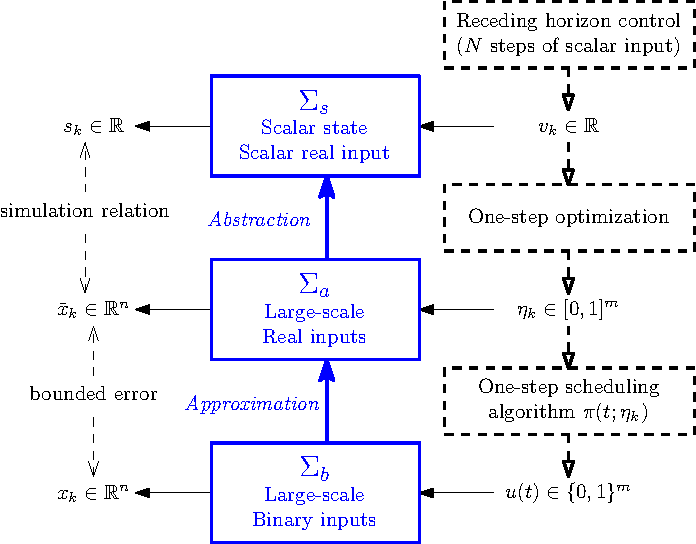
\includegraphics[width=\columnwidth]{approach_overview}
  \caption{Overview of the scheduling approach. The solid blue boxes represent the different models at different scales resulted from the offline design process: the original large-scale binary-input model $\Sigma_{b}$ is reduced to the single-state single-input model $\Sigma_{s}$.  The dashed boxes represent the run-time components, which include two lightweight optimizations and one simple scheduling algorithm.}
  \vspace{-10pt}
  \label{fig:overview}
\end{figure}

\begin{figure}[tb]
  \centering
  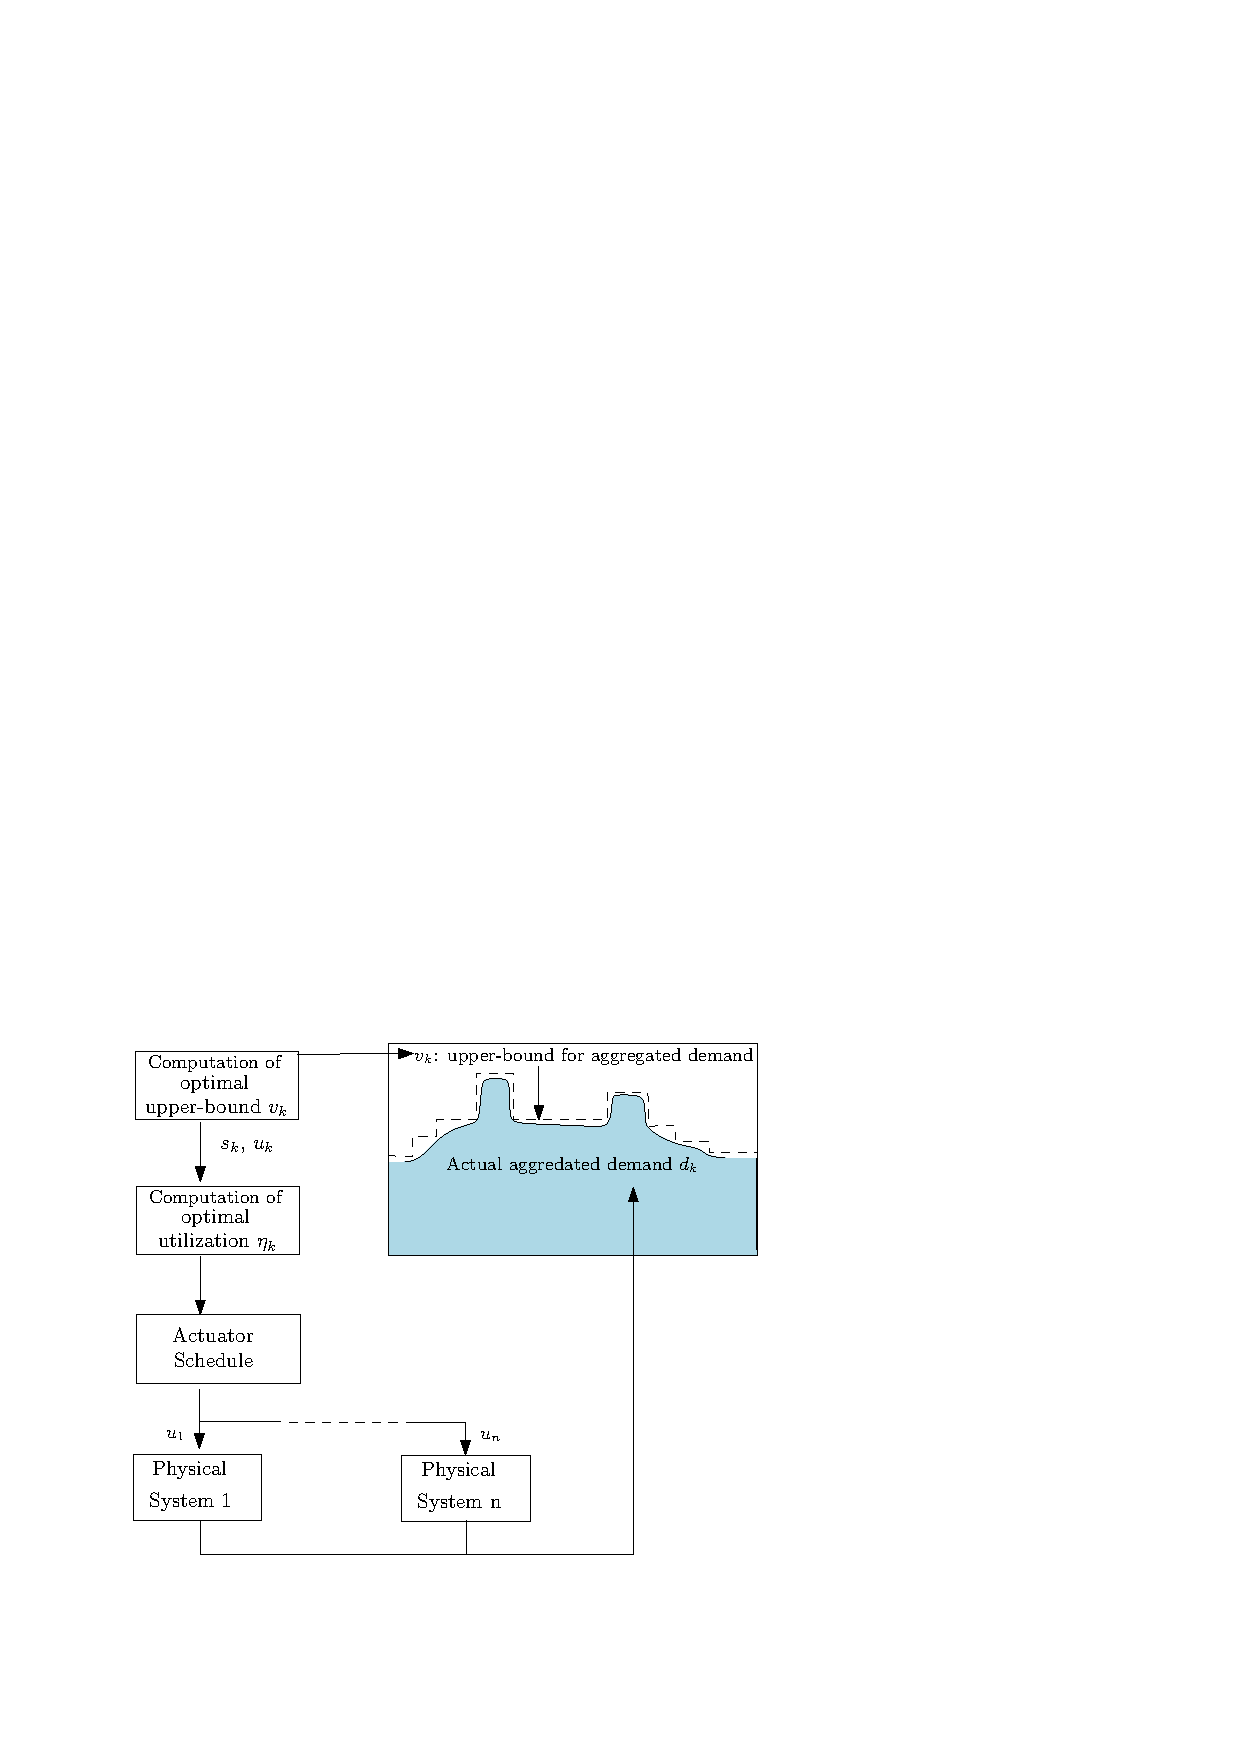
\includegraphics[width=\columnwidth]{runtime_hierarchy}
  \caption{Hierarchical control for minimizing aggregated energy cost across multiple subsystems.}% over a horizon.}
    \vspace{-10pt}
  \label{fig:runtime-hierarchy}
\end{figure}

The complexity of the %green
scheduling problem~\eqref{eq:GS-optim} comes mainly from the \emph{binary} control inputs $u$.
To alleviate this issue, we %relax 
approximate the original model $\Sigma_b$ by %considering
the averaged system $\Sigma_a$ with state $\overbar{x}$ for each time interval:
\begin{equation*}
(\Sigma_a) \qquad \dot{\overbar{x}} (t) = A \overbar{x} (t) + B \eta_k + Ew (t), \quad t \in [kT, (k + 1) T)
 \end{equation*}
where the control input $\eta_k = \frac{1}{T} \int_{kT}^{(k + 1) T} u (t) \mathd t$ is the \emph{average}, also called the \emph{utilization}, of $u (t)$ during the interval $[kT, (k + 1) T]$.
Clearly, $\eta_k$ is a vector of real numbers between $0$ and $1$: $\eta_k \in [0, 1]^m$.
Because the control input $\eta_k$ of $\Sigma_a$ is continuous, if we use $\Sigma_a$ in place of $\Sigma_b$, the complexity of the optimization is greatly reduced to that of an LP.
However, to ensure the safety constraint, we need to bound the deviation of $\overbar{x} (kT)$ from $x (kT)$ for all possible continuous-time binary input signals $u (t)$ that satisfy the utilization equation.
In Section~\ref{sec:averaged-system}, we will derive a tight bound on the error between $x$ and $\overbar{x}$.
As we will see, the error can be unbounded or become too large as $k$ increases, leading to overly conservative control inputs to ensure safety, or even infeasibility.
To keep this error as small as possible, we reset the state $\overbar{x}$ of $\Sigma_a$ to the measured state $x$ of $\Sigma_b$ at each $kT$, so that their error is reset to $0$.
Since the input $\eta_k$ is constant in each interval, $\Sigma_a$ can be discretized with sampling time $T$.
With the averaged system in place, we can reformulate the optimization~\eqref{eq:GS-optim} as minimizing the cost function~\eqref{eq:cost-function} subject to
\begin{subequations}
  \label{eq:averaged-optim}
  \begin{align}
    %\operatorname*{minimize}_{\eta_0, \ldots, \eta_{N - 1}} \quad & c_d \cdot \max_{0 \leqslant k \leqslant N - 1} d_k + \textstyle\sum_{0 \leqslant k \leqslant N - 1} c_{e, k} \cdot E_k  \label{eq:averaged-optim}\\
    %\text{subject to} \quad
    & \dot{x} (t) = Ax (t) + B \pi (t ; \eta_k) + Ew_{k} \quad \forall t \in [kT, (k + 1) T) %\forall t \geq 0 
\label{eq:averaged-optim:cont}\\
    %& u (t) = \pi (t ; \eta_k) \quad \forall t \in [kT, (k + 1) T) \label{eq:averaged-optim:control} \\ %, \quad \forall k = 0, \ldots, N - 1 \nonumber\\
    & A_{T}  \overbar{x}_{k} + B_{T} \eta_k + E_{T} w_{k} + e_{k+1} \in \XSet \quad \forall e_{k+1} \in \ESet (\eta_{k}) \label{eq:averaged-optim:safety}\\
    & \overbar{x}_{k} = x (kT) \label{eq:averaged-optim:reset}\\
    %& w (t) = w (kT) \in \mathcal{W} \quad \forall t \in [kT, (k + 1) T) \\
    & \eta_{k} \in [0,1]^{m}, \quad w_{k} \in \WSet, \quad E_k = Td_k, \quad d_k = \rho^T \eta_k
  \end{align}
\end{subequations}
where the constraints hold for all $k = 0, \ldots, N - 1$.
In the continuous-time dynamics~\eqref{eq:averaged-optim:cont}, $\pi (t ; \eta_k)$ is a scheduling algorithm that calculates the continuous-time schedule $u (t)$ during the $k$-th interval so that
its utilization is $\eta_k$.
%Such a scheduling algorithm is the topic of section \simpletodo{???Update???}
At each instant $kT$ the state $\overbar{x}_{k}$ of the averaged system is reset to the actual state $x (kT)$ (constraint~\eqref{eq:averaged-optim:reset}).
Let $e_{k+1}$ be the error between $x((k+1)T)$ and $\overbar{x}_{k}$, which is unknown but bounded in the $\eta_k$-dependent set $\ESet(\eta_{k})$ (\cf Section~\ref{sec:averaged-system}).
To ensure that $x (k T) \in \XSet$, constraint~\eqref{eq:averaged-optim:safety} robustly restricts the next state in $\XSet$ for all possible errors $e_{k+1}$.
%The utilization $\eta_{k}$, disturbance $w_{k}$ and the energy consumption $E_{k}$ and demand $d_{k}$ are constrained in 

%Except for the continuous-time dynamics~\eqref{eq:averaged-optim:cont}, problem~\eqref{eq:averaged-optim} is a linear program (LP).
In problem~\eqref{eq:averaged-optim}, the number of optimization variables $\eta_k \in \mathbbm{R}^m$, $k = 0, \ldots, N - 1$, is $mN$, which can be large for a large-scale system over a long horizon.
For instance, with $m=20$ control variables and sampling time $T = 5 \text{min}$ over a $24$-hour horizon, the number of optimization variables is $5 \comma 760$.
Constraint~\eqref{eq:averaged-optim:safety} involves high-dimensional dynamical equations and set operations over a long horizon, resulting in many constraints.
More importantly, constraint~\eqref{eq:averaged-optim:cont} requires execution of a continuous-time dynamical model.
%In particular, to robustly satisfy constraint~\eqref{eq:averaged-optim:safety}, the Pontryagin difference between $\XSet$ and the $\eta_{k}$-dependent set $\ESet(\eta_{k})$ must be computed every time the optimization 
For these reasons, problem~\eqref{eq:averaged-optim} is still difficult to solve, and its computational burden in run-time is still prohibitive for systems of practical size over a long horizon\footnote{In our targeted energy control applications, the horizon is typically a day, even a week or longer.}.
An embedded implementation of the controller is therefore unlikely realizable.
To reduce the complexity even further, we employ a \emph{model abstraction} technique based on the concept of simulation relations between transition systems \cite{aluretal00dah,girardetal07amd}.

A transition system is a generalization of a dynamical system, whose state can
transition into a new state either autonomously or under the influence of
exogenous inputs.
Intuitively speaking, a transition system $\mathcal{T}_2$ is said to {\emph{simulate}} another
transition system $\mathcal{T}_1$ if every move of $\mathcal{T}_1$ can be
tracked by $\mathcal{T}_2$ with respect to a symbolic relation between their states \cite{girardetal07amd}.
Formal definitions of transition systems and simulation relations will
be presented in Section~\ref{sec:abstraction}. The original definitions of a
simulation relation in the literature do not take into account %state and input constraints of each system, nor 
any relation between the two systems' inputs.
In this paper, we extend this concept so that $\mathcal{T}_2$ simulates
$\mathcal{T}_1$ while satisfying not only its state and input constraints but also a constraint between its input and that of $\mathcal{T}_1$.

Suppose that there exists a scalar discrete-time system:
\begin{align*}
(\Sigma_s) \quad
& s_{k + 1} = \alpha s_k + v_k + \beta^T w_{k} \\
& s_k \in \SSet \subseteq \mathbbm{R},
  v_k \in \VSet \subseteq \mathbbm{R},
  (s_k, v_k) \in \Omega \subseteq \SSet \times \VSet
\end{align*}
and a relation $\mathcal{R} \subseteq \mathcal{X} \times \mathcal{S}$ such
that $\Sigma_a$ simulates $\Sigma_s$ subject to the constraint $T \rho^{T} \eta_k
\leqslant v_k$ between their inputs. The intuition is that $s_k$ represents an
aggregated state of all the energy subsystems at time step $k$, and $v_k$ is
the total energy demand input to the system (more precisely, an upper-bound
thereof). Effectively, the scalar system $\Sigma_s$ abstracts the
higher-dimensional system $\Sigma_a$ by aggregating all the energy states and
inputs. The constraints $\mathcal{S}$, $\mathcal{V}$, and $\Omega$ are to
ensure compatibility with the state and input constraints of $\Sigma_a$. We
will show that any admissible trajectory of $\Sigma_s$ can be tracked by an
admissible trajectory of $\Sigma_a$ with equal or less energy cost (with
respect to the cost function~\eqref{eq:cost-function}). Therefore, instead
of solving the large-scale optimization \eqref{eq:averaged-optim}, we can
optimize the sequence of $\{ v_0, \ldots, v_{N - 1} \}$ for the scalar system
$\Sigma_s$, then recover the input $\eta_k$ by solving a simple optimization for
each time step $k$.
The benefit of our approach is that all the involved optimization
programs have much fewer variables and much less complexity, hence it is scalable.
This advantage is more significant when a receding horizon control approach is employed to
compute $\eta_k$ one step at a time.
In that case, we only solve two small-scale programs at each step, compared to a large-scale and  complex program if we solve \eqref{eq:averaged-optim} directly.
Details will be presented in the subsequent sections.

Our approach is best illustrated by Fig.~\ref{fig:overview}.
There are two processes involved:
\begin{itemize}
\item In the \textbf{offline} controller design process (blue boxes and text, left side, from bottom
  up) we start with the original system model
  $\Sigma_b$ and approximate it with the averaged system model $\Sigma_a$. The
  error bounds between the states of the two are also calculated as functions
  of $\eta_k$. Then $\Sigma_a$ is abstracted by a scalar system $\Sigma_s$,
  and a simulation relation $\RSet$ between them is constructed.
  
\item In the \textbf{online} controller execution process (dashed
  boxes, from top down) a receding horizon control
  framework is used with the abstract model $\Sigma_s$ to compute an
  optimal sequence of aggregate energy demands. Each energy demand
  $v_k$ is disaggregated into utilization values $\eta_k$ for the
  individual control inputs by a one-step optimization. A simple
  one-step scheduing algorithm $\pi$ schedules the subsystems so that
  each achieves the corresponding utilization.  This hierarchical control structure is illustrated in \cref{fig:runtime-hierarchy}.
\end{itemize}


%%% Local Variables:
%%% mode: latex
%%% TeX-master: "emsoft15gs"
%%% End:
